\section{Results}
\subsection{Basic verification and smooth accuracy}
The final test suite passes all 77 cases. The validation summary contains 25 checks, all passing. These include independent scalar-loop reproduction, analytic Fourier factors, exact shifts, invalid inputs and tolerance checks. The independent dense matrix exponential and FFT references agree within 5.551e-16. Basic PDE errors are reported in Table~\ref{tab:basic}; matching the reference is quantitative rather than based on curve overlap.
\begin{table}[htbp]\centering\small
\caption{Basic comparison at $N=200$, actual $C=0.5$, $T=0.25$. Exact shifted point samples are the reference. Source: joint\_convergence.csv.}\label{tab:basic}
\begin{tabular}{lllll}
\toprule
Datum & Method & $E_1$ & $E_2$ & $E_\infty$\\\midrule
sine & Upwind & 7.805e-03 & 8.670e-03 & 0.01226\\
sine & Lax--Wendroff & 1.234e-04 & 1.370e-04 & 1.938e-04\\
sine & MC & 5.724e-05 & 1.900e-04 & 1.178e-03\\
packet & Upwind & 0.0133 & 0.02735 & 0.1041\\
packet & Lax--Wendroff & 1.145e-03 & 2.476e-03 & 8.529e-03\\
packet & MC & 2.998e-04 & 1.298e-03 & 0.01194\\
square & Upwind & 0.03979 & 0.1078 & 0.4602\\
square & Lax--Wendroff & 0.02986 & 0.08947 & 0.5759\\
square & MC & 0.01206 & 0.05929 & 0.3801\\
\bottomrule\end{tabular}\end{table}
\begin{figure}[htbp]\centering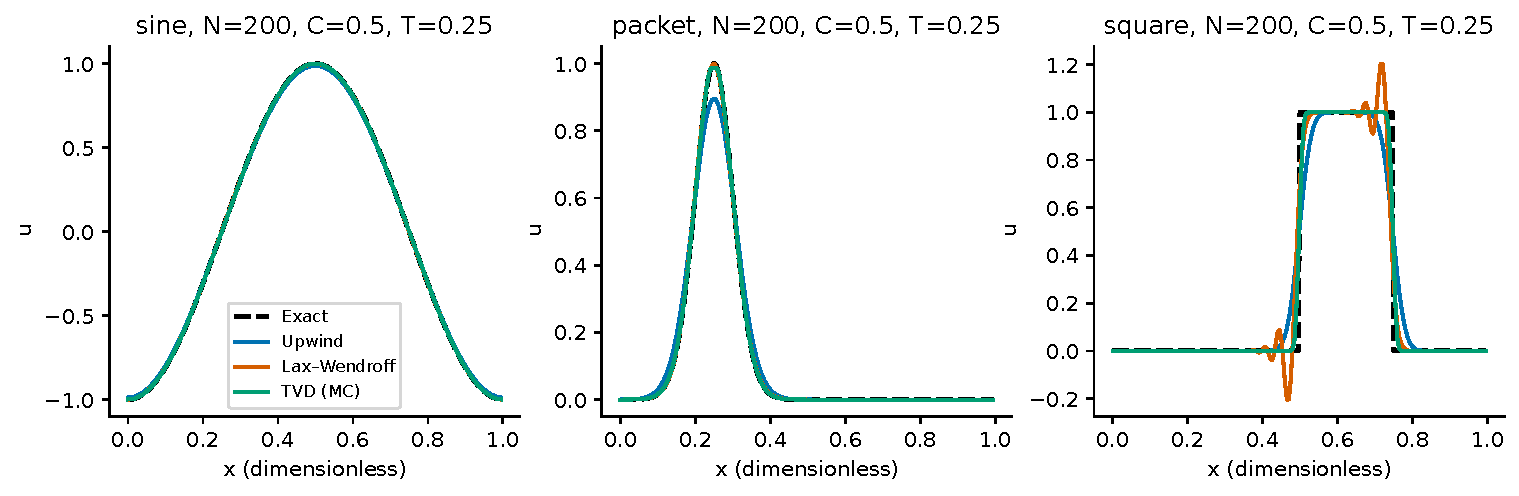
\includegraphics[width=.98\linewidth]{../results/figures/profiles.pdf}\caption{Exact and computed profiles at $N=200$, $C=0.5$, $T=0.25$. Every curve comes from the saved numerical arrays in profiles.npz. Upwind spreads the pulse; LW produces signed ripples; MC limits the jump correction.}\label{fig:profiles}\end{figure}
\subsection{What the separated studies actually measure}
Table~\ref{tab:space} removes time stepping from the spatial comparison. The upwind and central derivative limits approach orders one and two. MC's measured $L^2$ orders are lower than two. Limiting at smooth extrema affects an increasingly localized set, but its contribution can still dominate a global norm. This evidence supports local loss of order and rejects an unconditional claim that smooth data alone guarantee a global second-order MC rate.
\begin{table}[htbp]\centering\small
\caption{Separated spatial study, $T=0.1$, finest grid $N=800$ and order between $N=400$ and 800. Linear evolution is exact in time. MC uses the tolerance-refined limiting ODE.}\label{tab:space}
\begin{tabular}{lllll}
\toprule
Datum & Limit operator & $E_2$ & Finest pair order & Oracle change\\\midrule
sine & Upwind & 1.743e-03 & 0.9982 & 0.000e+00\\
packet & Upwind & 6.108e-03 & 0.9575 & 0.000e+00\\
sine & Lax--Wendroff & 4.568e-06 & 2 & 0.000e+00\\
packet & Lax--Wendroff & 8.284e-05 & 2 & 0.000e+00\\
sine & MC & 1.517e-05 & 1.733 & 2.169e-10\\
packet & MC & 1.117e-04 & 1.73 & 3.349e-10\\
\bottomrule\end{tabular}\end{table}
\begin{table}[htbp]\centering\small
\caption{Separated temporal study at fixed $N=100$, $T=0.1$, 1280 steps, relative to each same-grid small-step limit. The last order compares 640 and 1280 steps. It is not the joint PDE order.}\label{tab:time}
\begin{tabular}{lllll}
\toprule
Method & $\Delta t$ & Time $E_2$ & Last order & PDE spatial floor\\\midrule
Upwind & 7.813e-05 & 1.069e-04 & 1 & 0.01382\\
Lax--Wendroff & 7.813e-05 & 1.090e-07 & 1.056 & 2.923e-04\\
MC & 7.813e-05 & 7.691e-06 & 0.9961 & 6.000e-04\\
\bottomrule\end{tabular}\end{table}
The largest reference-tolerance change divided by a measured error is 7.897e-05, below the preregistered 0.01 contamination threshold. This empirical check makes unresolved reference error unlikely at the scale fitted, but does not turn the nonlinear ODE reference into an analytic oracle. For LW the temporal rate in Table~\ref{tab:time} approaches one, as predicted by \eqref{eq:lwtime}. Its PDE error is close to the fixed-grid spatial floor even while the smaller temporal discrepancy continues decreasing. Using the PDE error alone would obscure the temporal rate.
\begin{figure}[htbp]\centering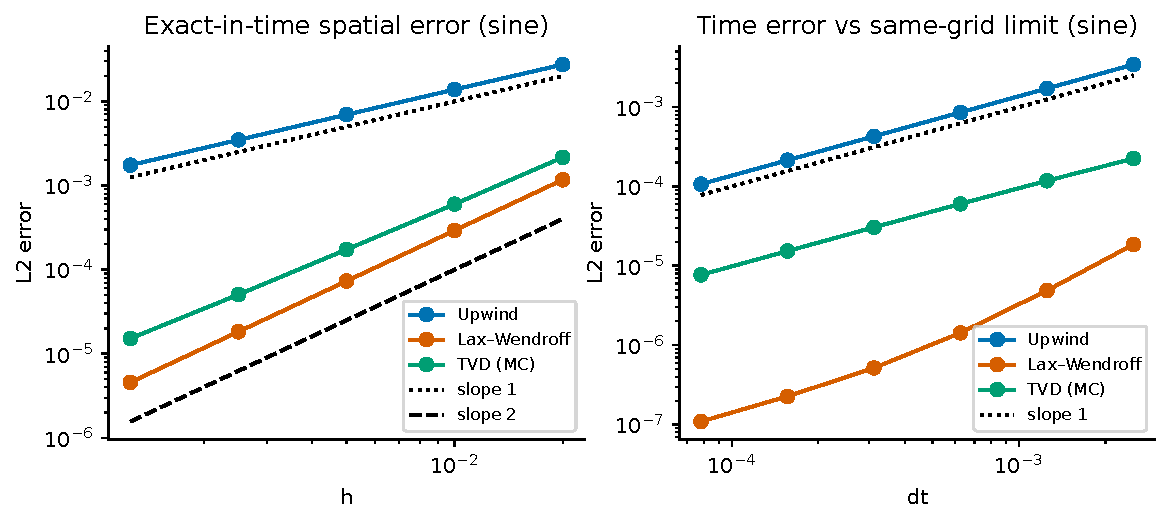
\includegraphics[width=.98\linewidth]{../results/figures/separated_convergence.pdf}\caption{Separated sine errors at $T=0.1$. Left: exact-in-time spatial operators against the PDE. Right: finite time stepping against each fixed-$N=100$ limiting system. Reference slopes identify the rate being measured.}\label{fig:sep}\end{figure}
\begin{figure}[htbp]\centering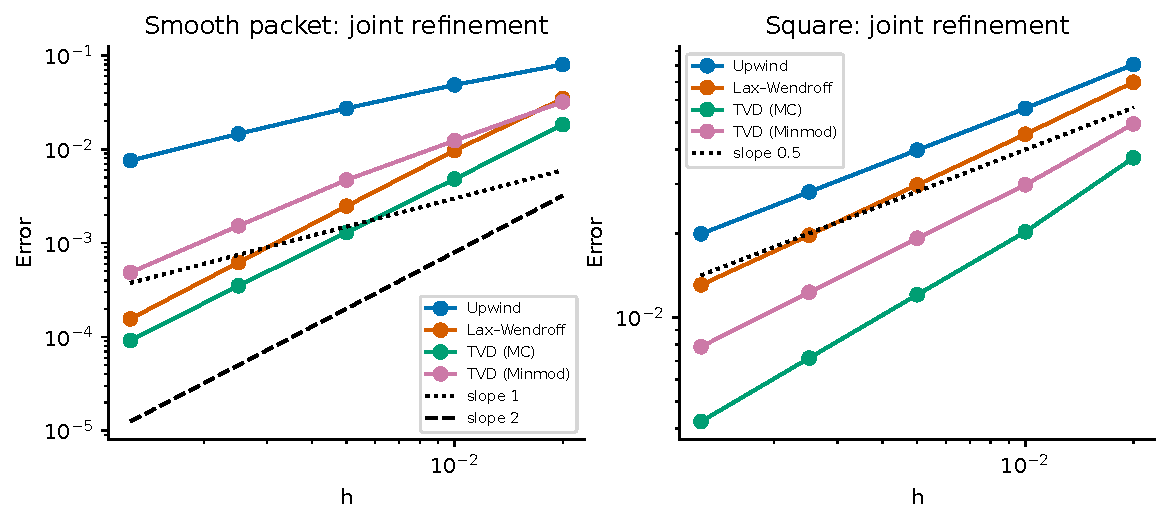
\includegraphics[width=.98\linewidth]{../results/figures/joint_convergence.pdf}\caption{Complete-format joint refinements at $C=0.5$, $T=0.25$. Left: smooth packet $L^2$ error. Right: square $L^1$ error. These are deliberately distinct from the separated studies. Minmod is a limiter sensitivity comparison.}\label{fig:joint}\end{figure}
\subsection{CFL boundary and spectral fidelity}
The checkerboard signed factors agree with the predictions to within 4.441e-16. At $C=1$ every tested method reduces to an exact represented shift. At $C=1.01$, the measured checkerboard amplitudes grow for both baselines; the more strongly unstable $C=1.1$ runs reach the explicit amplitude stop. In the limited checkerboard test all corrections vanish, so the measured factor is upwind's. This restricted experiment is consistent with the nonlinear analysis inside its CFL range and says little about arbitrary data outside it.
\begin{figure}[htbp]\centering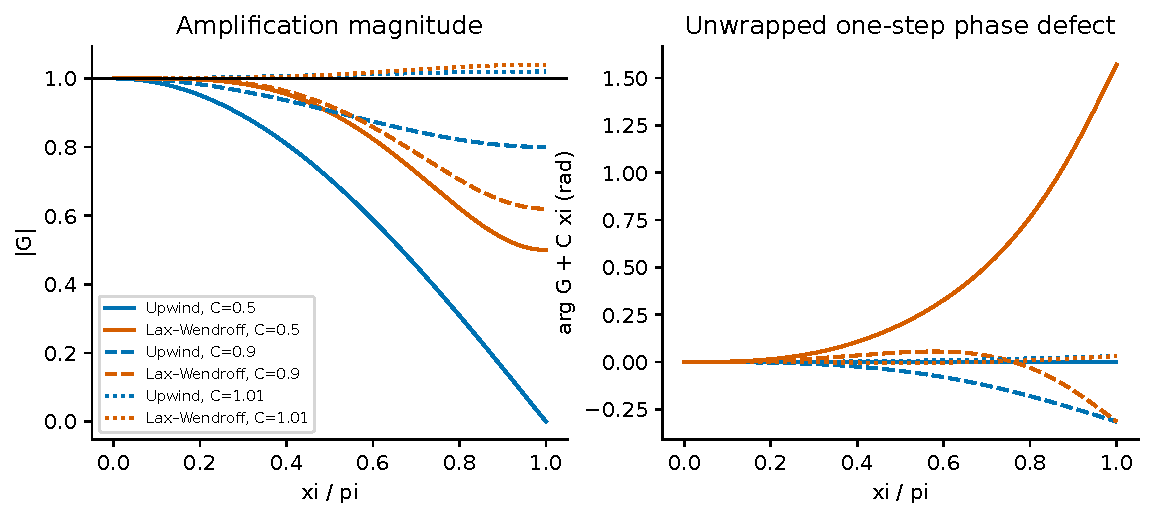
\includegraphics[width=.98\linewidth]{../results/figures/amplification.pdf}\caption{Linear baseline symbols on $0\le\xi\le\pi$. Magnitude and unwrapped one-step phase defect are different diagnostics. At high wave number the damping ordering can change with $C$. Phase at an exactly zero factor is masked.}\label{fig:amp}\end{figure}
\begin{figure}[htbp]\centering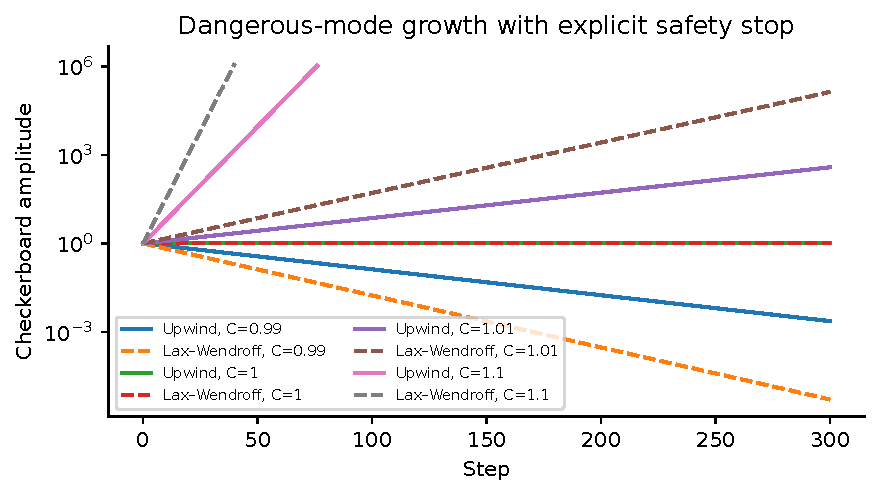
\includegraphics[width=.8\linewidth]{../results/figures/stability_growth.pdf}\caption{Dangerous checkerboard evolution on $N=100$, with CFL values around one. The explicit stress loop has a 300-step cap and a $10^6$ amplitude stop. Each curve records actual evolution rather than an arbitrary instability label.}\label{fig:stability}\end{figure}
Across the mode sweep, the maximum complex discrepancy between numerical projection and $G^{100}$ is 9.343e-15. At $C=0.5$ upwind can have essentially zero phase defect on the resolved branch yet strongly reduce amplitude. LW better preserves resolved amplitudes but accumulates a phase lag. This is why a single error measure cannot diagnose the mechanism.

MC's initial sine does not remain an exact single Fourier mode. Its original-mode coefficient measures effective amplitude and phase, and the CSV includes the residual outside that mode. These are measurements, not an asserted nonlinear amplification factor. For coefficients whose relative surviving amplitude is below $10^{-10}$, phase is flagged unreliable and numerical-speed points are omitted from the plot. Such computed phases remain in raw tables for audit, but support no speed claim.
\begin{figure}[htbp]\centering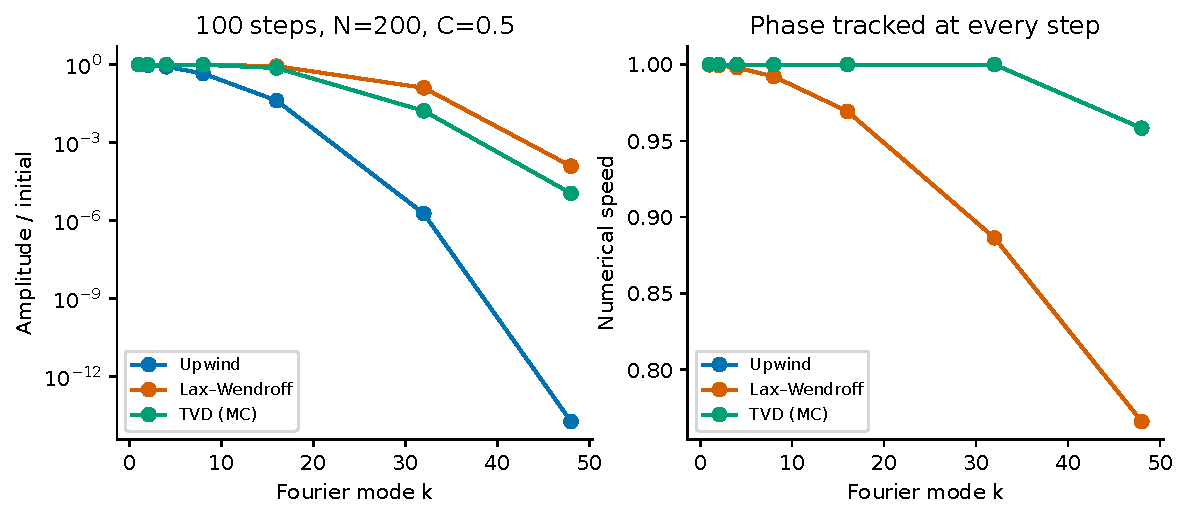
\includegraphics[width=.98\linewidth]{../results/figures/modal_fidelity.pdf}\caption{Actual modal projections after 100 steps at $N=200$, $C=0.5$. Linear predictions are separately checked in fourier\_modes.csv. MC points are measured effective responses. Speed values below the amplitude reliability gate are omitted.}\label{fig:modal}\end{figure}
\subsection{Discontinuous pulse, transition widths and limiter sensitivity}
\begin{table}[htbp]\centering\small
\caption{Square at $N=200$, $C=0.5$, $T=0.25$. Initial TV is 2. Cells count both threshold transition regions; the aggregate physical width equals count divided by 200.}\label{tab:square}
\begin{tabular}{lllllll}
\toprule
Method & $E_1$ & $E_\infty$ & Overshoot & Undershoot & TV & Cells\\\midrule
Upwind & 0.03979 & 0.4602 & 0.000e+00 & 0.000e+00 & 2 & 24\\
Lax--Wendroff & 0.02986 & 0.5759 & 0.2041 & 0.2041 & 3.446 & 12\\
MC & 0.01206 & 0.3801 & 0.000e+00 & 0.000e+00 & 2 & 8\\
Minmod & 0.01924 & 0.4033 & 0.000e+00 & 0.000e+00 & 2 & 12\\
\bottomrule\end{tabular}\end{table}
LW's negative stencil weight permits overshoot and undershoot. Its TV can exceed the exact value despite its proved $L^2$ stability. MC suppresses these extrema within the tested tolerances while spreading the jump across several cells. Minmod trades additional spreading for more restrictive slopes. Neither limiter eliminates numerical error.

A diffusion balance explains upwind's square-pulse behavior: its modified viscosity is proportional to $h$ at fixed $C$, so a transported front has physical thickness proportional to $\sqrt{hT}$. The number of cells across it consequently grows like $h^{-1/2}$ even as its physical width shrinks. This supports the approximately half-order $L^1$ behavior and explains why rising discrete $L^\infty$ error is compatible with convergence in $L^1$. Values adjacent to a moving jump remain mixtures of the two states. The discrete maximum norm exposes that transition, but cannot substitute for measuring its width.
\begin{table}[htbp]\centering\small
\caption{Finest square grid $N=800$, $C=0.5$, $T=0.25$. Threshold width includes both fronts. All jump references follow the same half-open point convention.}\label{tab:squarefine}
\begin{tabular}{llllll}
\toprule
Method & $E_1$ & $E_2$ & $E_\infty$ & Physical width & Cells\\\midrule
Upwind & 0.01993 & 0.07638 & 0.4801 & 0.065 & 52\\
Lax--Wendroff & 0.01308 & 0.05858 & 0.6111 & 0.0275 & 22\\
MC & 4.237e-03 & 0.03572 & 0.4149 & 0.015 & 12\\
Minmod & 7.852e-03 & 0.04594 & 0.4382 & 0.025 & 20\\
\bottomrule\end{tabular}\end{table}
\begin{table}[htbp]\centering\small
\caption{Limiter sensitivity across requested Courant numbers 0.25, 0.5 and 0.9, at $N=200$, $T=0.25$. The table reports actual $C$ after uniform endpoint adjustment.}\label{tab:limiterC}
\begin{tabular}{llllll}
\toprule
Datum & Limiter & Actual $C$ & $E_1$ & $E_\infty$ & TV\\\midrule
packet & MC & 0.25 & 5.548e-04 & 0.01388 & 1.972\\
packet & MC & 0.5 & 2.998e-04 & 0.01194 & 1.976\\
packet & MC & 0.8929 & 1.259e-04 & 4.603e-03 & 1.991\\
packet & Minmod & 0.25 & 2.269e-03 & 0.03971 & 1.921\\
packet & Minmod & 0.5 & 1.612e-03 & 0.03073 & 1.939\\
packet & Minmod & 0.8929 & 3.653e-04 & 0.0103 & 1.979\\
square & MC & 0.25 & 0.01354 & 0.4118 & 2\\
square & MC & 0.5 & 0.01206 & 0.3801 & 2\\
square & MC & 0.8929 & 8.130e-03 & 0.3406 & 2\\
square & Minmod & 0.25 & 0.02233 & 0.4288 & 2\\
square & Minmod & 0.5 & 0.01924 & 0.4033 & 2\\
square & Minmod & 0.8929 & 0.01094 & 0.3474 & 2\\
\bottomrule\end{tabular}\end{table}
The limiter sweep in Table~\ref{tab:limiterC} holds the mesh, datum and physical time fixed while changing the Courant number. Its variation reflects both the correction prefactor $(1-C)$ and the changed number of limiting operations. Minmod is generally more restrictive, but a smaller phase or maximum error is not guaranteed by a TVD inequality. Endpoint adjustment matters: the requested 0.9 case need not execute at exactly 0.9. All all-step TV conclusions use the actual executed step.
\begin{figure}[htbp]\centering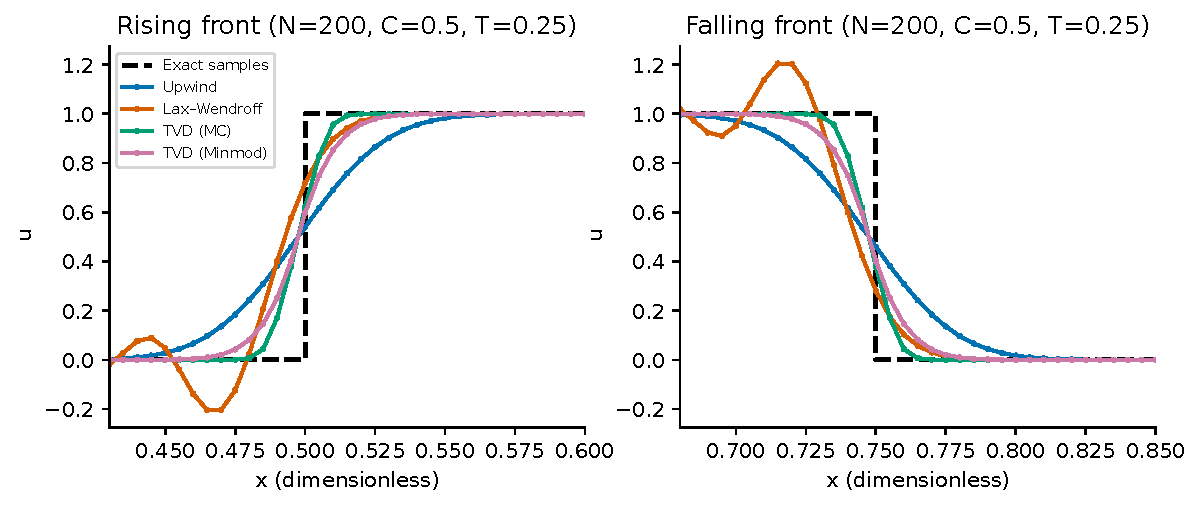
\includegraphics[width=.98\linewidth]{../results/figures/square_zoom.pdf}\caption{Local views of both square fronts at $N=200$, $C=0.5$, $T=0.25$. Markers show stored point values. The exact display joins half-open samples with steps and is not used as an interpolated reference for error norms.}\label{fig:zoom}\end{figure}
\subsection{Mass and total variation histories}
Over all diagnostic runs, the maximum absolute mass residual is 1.776e-16. MC's maximum single-step TV increment is 8.882e-16, below the declared $5\times10^{-12}$ tolerance. These checks include the periodic seam, three profiles and three requested Courant numbers. Roundoff-scale positive increments are reported rather than rounded into an assertion of exact monotonicity in floating-point arithmetic. The mathematical TVD proof is independent of the sampled experiment.

Conservation is shared by all methods. It therefore cannot select the most accurate method: the mass time series is nearly unchanged even when the square profile is smeared or oscillatory. The histories also provide minima and maxima at every step rather than just a favorable final snapshot.
\begin{figure}[htbp]\centering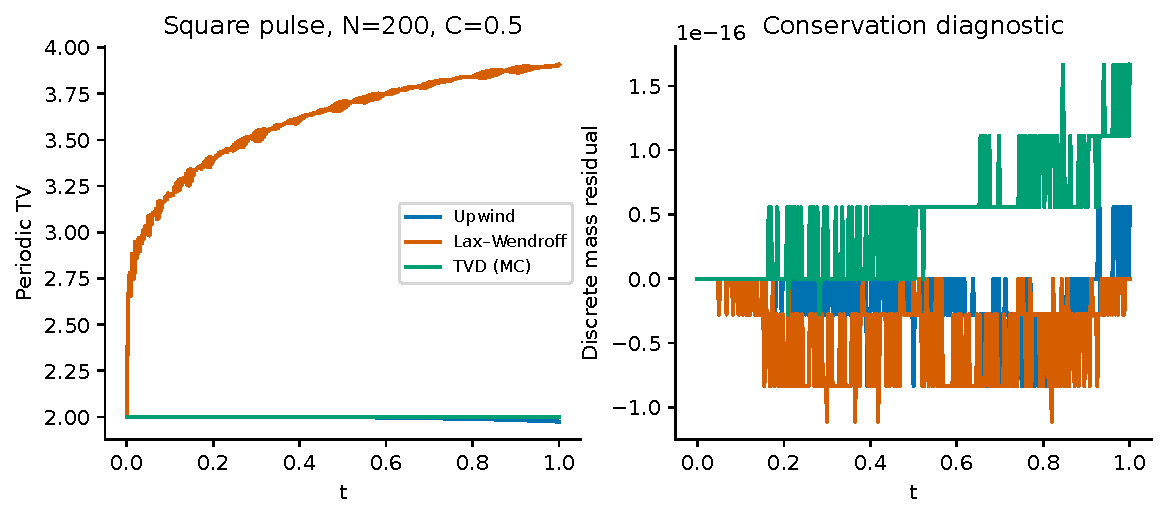
\includegraphics[width=.98\linewidth]{../results/figures/mass_tv.pdf}\caption{Square diagnostic histories for $N=200$, $C=0.5$, $0\le t\le1$. Periodic TV distinguishes oscillatory behavior while discrete mass remains conserved. The scale of the mass panel is numerical roundoff.}\label{fig:tv}\end{figure}
\subsection{Long-time accumulation}
\begin{table}[htbp]\centering\small
\caption{Sine after ten periods at $N=200$, $C=0.5$. Phase is accumulated from consecutive stored steps. Additional $T=0.37,1.37,5.37$ diagnostics remove ambiguity from viewing only return times.}\label{tab:long}
\begin{tabular}{lllll}
\toprule
Method & $E_2$ & Amplitude ratio & Phase defect (rad) & Mass residual\\\midrule
Upwind & 0.2754 & 0.6105 & -7.105e-15 & -1.776e-16\\
Lax--Wendroff & 5.481e-03 & 0.9999 & 7.751e-03 & -3.553e-17\\
MC & 1.333e-03 & 0.9999 & 7.105e-15 & -2.487e-16\\
\bottomrule\end{tabular}\end{table}
Upwind accumulates damping even where its resolved-mode phase at $C=0.5$ is exact. LW accumulates a measurable phase defect with much smaller amplitude loss. Limitation changes waveform shape and introduces harmonics, so MC's coefficient describes only the original mode. Intermediate diagnostics and unwrapped histories prevent a phase change by an integer multiple of $2\pi$ from masquerading as zero phase error. The complete CSV includes all three profiles and Minmod sensitivity, not only the sine figure.
\begin{figure}[htbp]\centering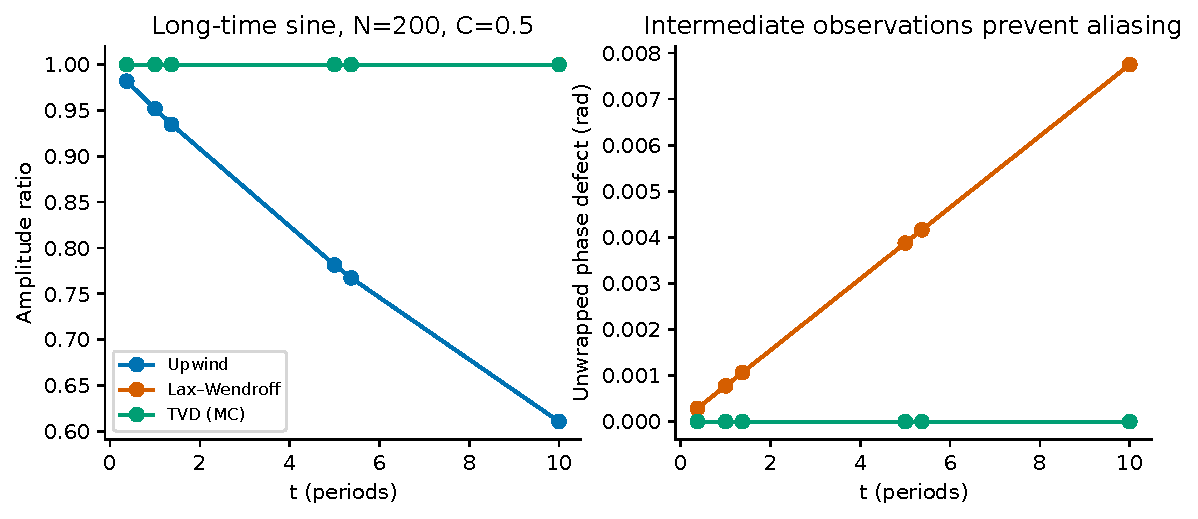
\includegraphics[width=.98\linewidth]{../results/figures/long_time.pdf}\caption{Amplitude and unwrapped phase of the sine over up to ten transit periods. Identical $N=200$ and $C=0.5$ provide equal physical times and mesh conditions. Additional nonreturn times support phase interpretation.}\label{fig:long}\end{figure}
\subsection{Cost at matched accuracy}
We predeclared $L^1$ targets 0.02 and 0.005 for the packet, and 0.05 and 0.02 for the square. Each method searches the same $N=50,100,\ldots,3200$ set at $C=0.5$, $T=0.25$. One warmup precedes seven timed repetitions. Timing includes state copy, driver checks, allocations and stepping, and excludes imports, diagnostics, parameter search, file writes and plotting. We report median and interquartile range (IQR). Small runtimes are sensitive to background scheduling; all individual samples are archived. Grid updates complement wall-clock cost but do not equate the work per update across methods.
\begin{table}[htbp]\centering\small
\caption{Matched-target packet configurations. Each row is the fastest \emph{measured} satisfying configuration for that method on the tested grid set. Actual $\Delta t$ and grid updates are in matched\_targets.csv.}\label{tab:costpacket}
\begin{tabular}{lllllll}
\toprule
Method & Target & $N$ & Steps & Measured $E_1$ & Median (s) & IQR (s)\\\midrule
Upwind & 0.02 & 200 & 100 & 0.0133 & 4.538e-04 & 2.425e-05\\
Upwind & 5.000e-03 & 800 & 400 & 3.609e-03 & 2.124e-03 & 5.548e-05\\
Lax--Wendroff & 0.02 & 50 & 25 & 0.01681 & 6.475e-04 & 1.681e-04\\
Lax--Wendroff & 5.000e-03 & 100 & 50 & 4.525e-03 & 9.398e-04 & 1.271e-04\\
MC & 0.02 & 50 & 25 & 7.164e-03 & 4.602e-04 & 8.896e-06\\
MC & 5.000e-03 & 100 & 50 & 1.534e-03 & 9.217e-04 & 1.100e-05\\
\bottomrule\end{tabular}\end{table}
\begin{table}[htbp]\centering\small
\caption{Matched-target square configurations. Each row is the fastest \emph{measured} satisfying configuration for that method on the tested grid set. Actual $\Delta t$ and grid updates are in matched\_targets.csv.}\label{tab:costsquare}
\begin{tabular}{lllllll}
\toprule
Method & Target & $N$ & Steps & Measured $E_1$ & Median (s) & IQR (s)\\\midrule
Upwind & 0.05 & 200 & 100 & 0.03979 & 4.664e-04 & 1.265e-05\\
Upwind & 0.02 & 800 & 400 & 0.01993 & 2.022e-03 & 5.425e-05\\
Lax--Wendroff & 0.05 & 100 & 50 & 0.04535 & 8.142e-04 & 5.563e-06\\
Lax--Wendroff & 0.02 & 400 & 200 & 0.01971 & 3.459e-03 & 6.108e-05\\
MC & 0.05 & 50 & 25 & 0.03734 & 4.889e-04 & 5.353e-06\\
MC & 0.02 & 200 & 100 & 0.01206 & 2.056e-03 & 6.365e-05\\
\bottomrule\end{tabular}\end{table}
For the final recorded timing run, the fastest satisfying methods across the tested configurations are Upwind for packet at target 0.02, MC for packet at target 0.005, Upwind for square at target 0.05, Upwind for square at target 0.02. These are environment-specific observations rather than universal complexity claims. All declared targets were achieved in the tested set. The code records nonachievement explicitly if a future run or changed target has no satisfying configuration.
\begin{figure}[htbp]\centering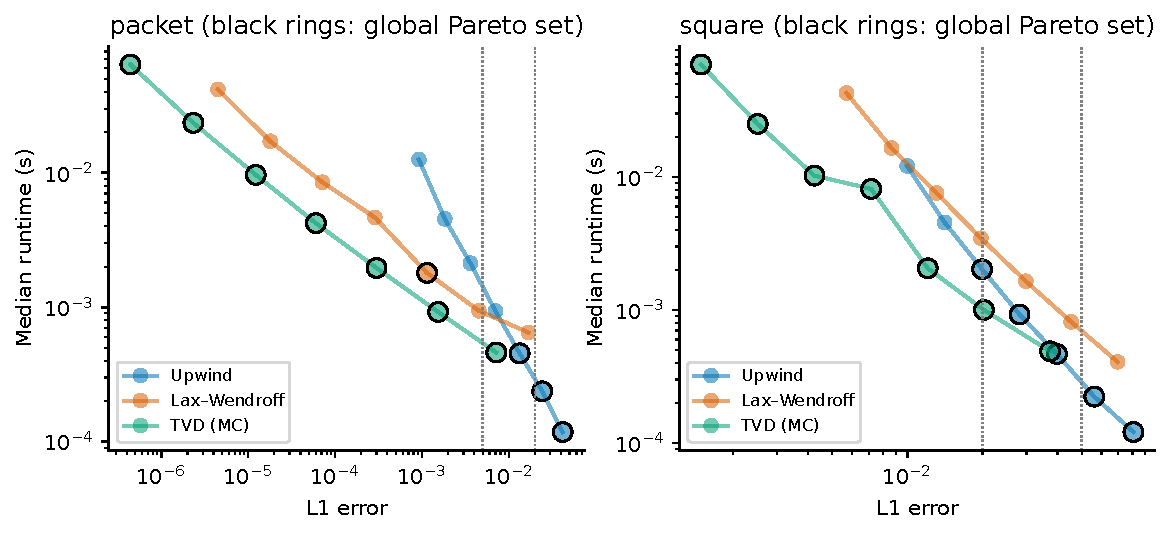
\includegraphics[width=.98\linewidth]{../results/figures/cost_accuracy.pdf}\caption{Cost--accuracy curves at $C=0.5$, $T=0.25$. Black rings mark the nondominated set across all methods for each datum; dotted vertical lines mark declared targets. Pareto membership uses measured medians and errors, and can vary with timing noise.}\label{fig:cost}\end{figure}
\section{Discussion}
The mechanisms predict different advantages. Upwind's convex weights provide robust extrema control at the cost of first-order diffusion. LW's correction removes the leading diffusion and substantially lowers smooth error, but its negative coefficient permits ripples at jumps. The limited flux restricts that correction where adjacent gradients disagree, controlling total variation while retaining a sharper pulse than upwind in the representative square comparison. This mechanism explains the observed tradeoff without assuming that an advanced method wins every metric.

The choice of norm is part of the question. A method can have smaller $L^1$ error while violating a range constraint that matters in an application. Conversely, a TVD solution can preserve bounds while clipping smooth extrema and producing a larger global error. At $N=200$, $C=0.5$, $T=0.25$, the square $L^1$ errors of LW and MC are 0.02986 and 0.01206 respectively. Their extrema and TV give additional information beyond that scalar ranking. At the same configuration for the sine, MC has $L^1$ error 5.724e-05 versus LW's 1.234e-04, but MC's $L^2$ error is 1.900e-04 versus LW's 1.370e-04. Thus the norm alone changes that comparison. TVD is a structural inequality, with no theorem ordering $\|U-u\|$ against LW or upwind.

CFL sensitivity is also substantive. As $C\to1$, the baseline modified-error coefficients decrease; $C=1$ is an exact shift of the represented state. It would make an artificially favorable primary comparison. Our interior-CFL sweeps retain the balance between damping and dispersion, and the square tables record actual CFL after endpoint adjustment. The method recommended at one error target may change when the datum, tolerance, or a no-overshoot constraint changes. Timings alone at a common grid cannot answer that question.

The benchmark contains no measured-data mismatch. A physical reduction to one-dimensional constant-speed transport would omit diffusion, variable velocity, boundaries and reactions. Those modelling errors cannot be estimated from exact-shift agreement here. No inference about general nonlinear conservation laws, shocks in gas dynamics, or real-world predictive validity is supported.

\section{Limitations and remaining human responsibilities}
The study covers one dimension, a constant coefficient, a periodic uniform grid and selected finite resolutions. Smooth Taylor and Fourier expansions are inapplicable directly at jumps. Nonlinear reference separation relies on a tolerance-refined ODE computation rather than a certified analytic solution; limiter switches can affect adaptive integration. The observation of a rate is empirical and is not a general convergence proof. Transition width depends on its 0.1--0.9 threshold, and for oscillatory profiles includes ripple values. A larger grid set and multiple timing sessions would better resolve close cost rankings. Seven short timings in one process do not quantify all system variability.

There is no supplied standalone rubric, official LaTeX source template, presentation duration, syllabus calendar or live submission checklist in the local pack. Tutorial 13 states a LaTeX report of at least eight pages. We follow that constraint with an article report and a Beamer presentation. Brief and real-world pack say Monday of Week 15, while Lecture 5 says Week 14. We prioritize the Brief and flag the discrepancy for the team to resolve against the published calendar; no calendar date is invented.

The named one-page Problem Definition Sheet was typeset after the first experiment run, although its mathematical specification and hypotheses already appeared in the preregistered protocol. This is a disclosed process deviation. The full run command was rerun after software integration and phase-gating corrections. The official teammate clean-room check, peer challenge, role handover, forum milestones, repository invitations, individual contribution statements and viva ownership remain human actions. They cannot be generated as historical facts by an agent. This deliverable is an AI-assisted reference study with six named ICS templates, not evidence that those requirements have been performed.

\section{Conclusion}
The verified baselines expose a clear distinction between dissipation, dispersion and instability. Upwind sacrifices amplitude and transition sharpness for convex, conservative transport. LW gains smooth accuracy while allowing bounded dispersive ripples. MC controls periodic total variation and range under the proved CFL condition, with additional computation and loss of accuracy near smooth extrema. Its empirical spatial rate in the selected norm is below two, which is a meaningful result rather than a failed attempt to recover a preferred order.

Exact same-grid references show why fixed-CFL joint refinement is insufficient to identify time order. Classical LW approaches its central semidiscrete limit at first order in time on a fixed mesh, while maintaining second-order smooth PDE accuracy on hyperbolic refinement families. This distinction is central to the evidence chain. Matched-target timings and Pareto curves connect numerical quality to cost without asserting a universal winner. The next decisive computational check would repeat the matched-target benchmark in an independently created teammate environment and compare both numerical outputs and timing uncertainty.
